Given that the product we want to study generates more interest in women rether than in men, we decided to focus our studies on women only. We also came to the conclusion that since a luxury scarf is usually bought from the middle and the upper class person, a minimum family yearly income bound was necessary to set our focus on only the users that are able to generate more impact on the analysis. We set this bound at 80.000 \EUR{} gross. Finally we thought that since trends can vary among countries, considering only the Italian population was the most reasonable choice to avoid unwanted biases.
The binary features that we decided to observe on our users are:
\begin{itemize}
	\item \textbf{With/Without children}:\@ To better observe the impact that a son can have in buying a luxury item
	\item \textbf{Living in the North/South of Italy}:\@ To better observe the impact that the climate and the local traditions can have in buying an item that is useful only in certain seasons.
\end{itemize}
The distribution of our customer base is described in the following pie chart:
\makebox[\textwidth][c]{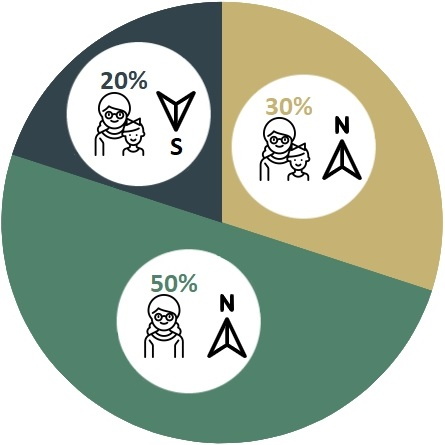
\includegraphics[width=0.7\textwidth]{sections/images/usersImage3}}
%\makebox[\textwidth][c]{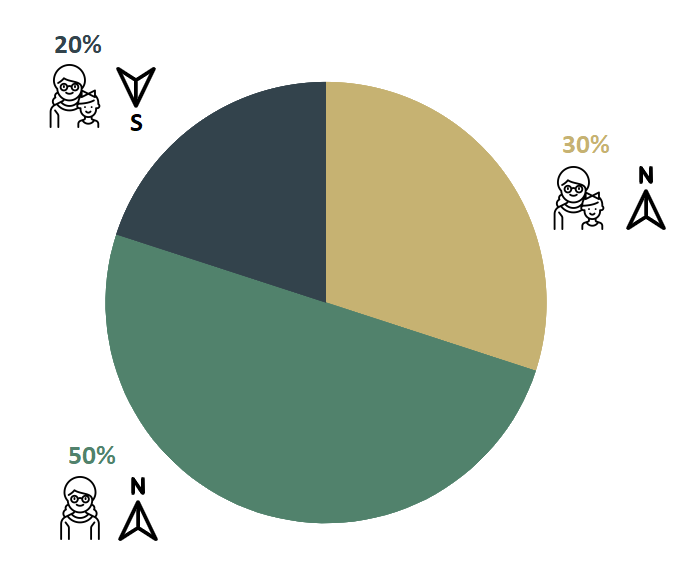
\includegraphics[width=0.9\textwidth]{sections/images/usersImage}}